\newpage
\section{Ley de Benford}
\subsection{Introducción}
En 1981, Simon Newcomb publicó un art\'iculo que comienza diciendo que la
frecuencia de aparición de los 10 dígitos en algún número no era equitativa y
que esto debía ser evidente al observar las tablas de logaritmos y notar que las
primeras p\'aginas estaban m\'as que las del final. Esto result\'o para Newcomb
en el siguiente enunciado:

\textit{La ley de probabilidad de ocurrencia de los n\'umeros es tal que la mantisa 
de su logaritmo es equiprobable.}

Despu\'es de estos resultados, en 1937, Frank Benford retoma los resultados de
Newcomb y publica su \textit{Ley de los n\'umeros an\'omalos}.

El m\'etodo de estudio consiste en seleccionar cualquier tabla de datos que no
esté restringida en rango numérico o condicionada de alguna manera y hacer el
conteo del n\'umero de veces que los n\'umeros naturales del 1 al 9 curren como
primer dígito. Si aparece un punto decimal o un cero antes del primer n\'umero
natural, estos deben ser ignorados.
\subsection{Ley para n\'umeros grandes}
Para comrpobar su hip\'otesis, Benford recolectó informaci\'on de distintas
fuentes. Estos datos se encuentran naturalmente de forma aleatoria. Una vez que
realizó el conteo de aproximadamente 20,229 observaciones, obtuvo el promedio de
apariciones de cada dígito en la primera posici\'on de los n\'umeros
Fig. (\ref{T1Benford}). 

\begin{figure}[h]
	\centering
	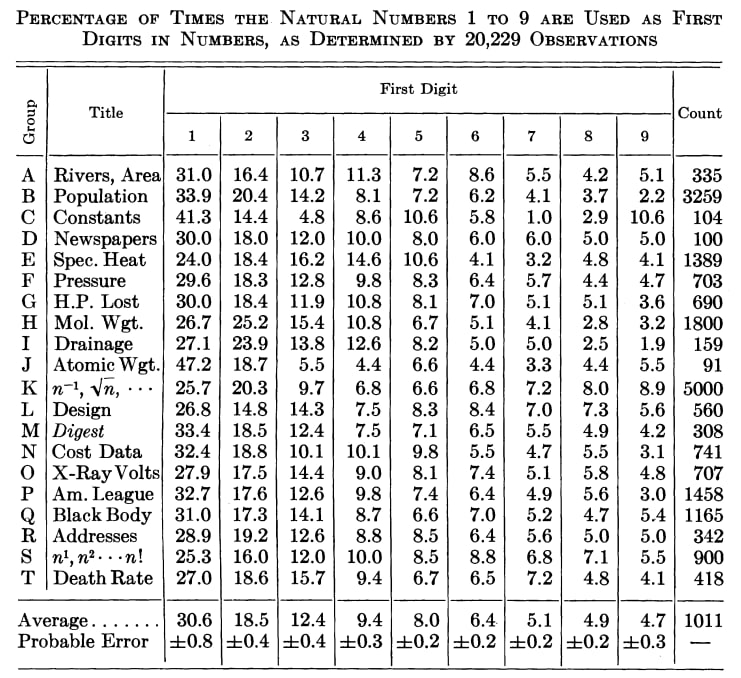
\includegraphics[scale=0.4]{figures/benford_table.jpg}
	\caption{Tabla de porcentajes de aparici\'on de los n\'umeros naturales para diferentes experimentos.}
	\label{T1Benford}
\end{figure}

\begin{figure}[h]
	\centering
	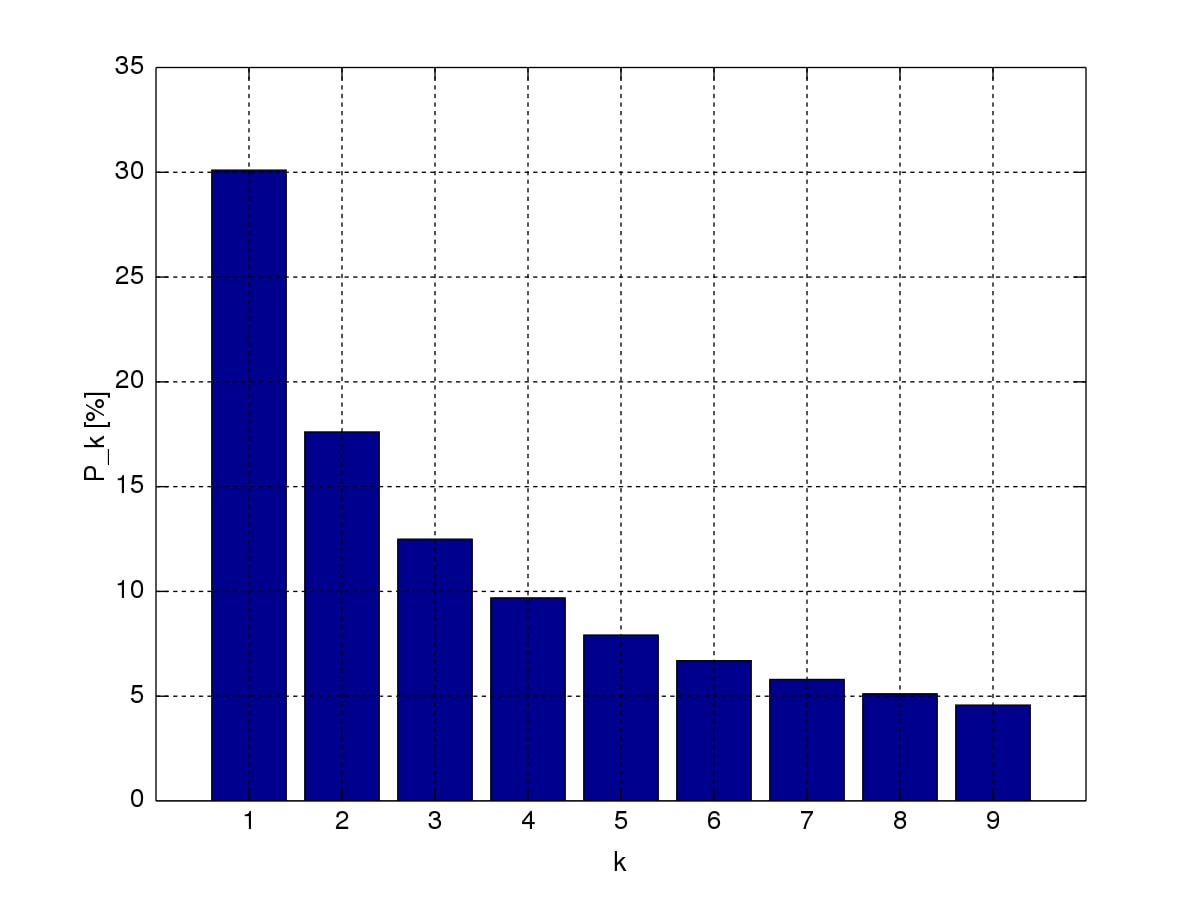
\includegraphics[scale=0.4]{figures/benford_frequency.jpg}
\caption{Gr\'afica de comportamiento para la Ec\eqref{BenfordFrecuency}.}
	\label{G1Benford}
\end{figure}
De la Fig. (\ref{T1Benford}), si se toma el promedio final de cada columna y se
estudia, por ejemplo, el 0.306, en lugar de 30.6. Se debe notar que la
frecuencia de aparici\'on del 1 como primer dígito es equivalente a $log 2$;
mientras que la frecuencia de aparici\'on del 2 como primer d\'igito (promedio
0.185), es igual al $log 3-log 2$ Ec.\eqref{BenfordFrecuency}. Este
comportamiento persiste hasta el promedio de la columna 10, donde 0.047 es
equivalente al $log \frac{10}{9}$.

Así, la frecuencia con la que aprece cada uno de los 9 n\'umeros como primer
d\'igito est\'a dada por la Ec.\eqref{BenfordFrecuency}. Mientras que en la
Fig. (\ref{G1Benford}) se muestra la gr\'afica de comportamiento de la frecuencia
con la que aparece cada uno de los n\'umeros como primer d\'igito.
\begin{equation}
	F_a=log(\frac{a+1}{a})
	\label{BenfordFrecuency}
\end{equation}

\subsection{Comportamiento para la q-\'esima posici\'on}
En el caso de la frecuencia de aparici\'on de cada d\'igito como segunda
posici\'on, el cero debe ser contemplado, así como el d\'igito $a$ de la primera
posici\'on. De acuerdo con un sistema posicional, sea $ab$ el n\'umero formado
por el d\'igito de la posici\'on 1 y 2, respectivamente. 

De acuerdo con la Ec.\eqref{BenfordFrecuency}, La frecuencia de aparici\'on del
n\'umero compuesto como primer n\'umero es
\begin{equation}
	F_ab=log (\frac{ab+1}{ab})
\end{equation}
Sin embargo, no se ha considerado la probabilidad de $a$ en la primer posici\'on
de $ab$. Por lo tanto, el problema se puede modelar de forma similar a una
probabilidad condicional: $P(ab|a)$. De esta forma, se tiene la siguiente
expresi\'on
\begin{equation}
	F_b=\frac{log (\frac{ab+1}{ab})}{log(\frac{a+1}{a})}
\end{equation}
De forma m\'as general...
\begin{equation}
	F_q=\frac{log(\frac{(abc...pq)+1)}{abc...pq})}{log(\frac{(abc...op)+1}{abc...p})}
\end{equation}